% Options for packages loaded elsewhere
\PassOptionsToPackage{unicode}{hyperref}
\PassOptionsToPackage{hyphens}{url}
\PassOptionsToPackage{dvipsnames,svgnames*,x11names*}{xcolor}
%
\documentclass[
]{article}
\usepackage{amsmath,amssymb}
\usepackage{lmodern}
\usepackage{ifxetex,ifluatex}
\ifnum 0\ifxetex 1\fi\ifluatex 1\fi=0 % if pdftex
  \usepackage[T1]{fontenc}
  \usepackage[utf8]{inputenc}
  \usepackage{textcomp} % provide euro and other symbols
\else % if luatex or xetex
  \usepackage{unicode-math}
  \defaultfontfeatures{Scale=MatchLowercase}
  \defaultfontfeatures[\rmfamily]{Ligatures=TeX,Scale=1}
\fi
% Use upquote if available, for straight quotes in verbatim environments
\IfFileExists{upquote.sty}{\usepackage{upquote}}{}
\IfFileExists{microtype.sty}{% use microtype if available
  \usepackage[]{microtype}
  \UseMicrotypeSet[protrusion]{basicmath} % disable protrusion for tt fonts
}{}
\makeatletter
\@ifundefined{KOMAClassName}{% if non-KOMA class
  \IfFileExists{parskip.sty}{%
    \usepackage{parskip}
  }{% else
    \setlength{\parindent}{0pt}
    \setlength{\parskip}{6pt plus 2pt minus 1pt}}
}{% if KOMA class
  \KOMAoptions{parskip=half}}
\makeatother
\usepackage{xcolor}
\IfFileExists{xurl.sty}{\usepackage{xurl}}{} % add URL line breaks if available
\IfFileExists{bookmark.sty}{\usepackage{bookmark}}{\usepackage{hyperref}}
\hypersetup{
  pdftitle={Meta-análisis en R},
  pdfauthor={Juan David Leongómez1,},
  colorlinks=true,
  linkcolor=black,
  filecolor=Maroon,
  citecolor=Blue,
  urlcolor=blue,
  pdfcreator={LaTeX via pandoc}}
\urlstyle{same} % disable monospaced font for URLs
\usepackage[margin=2cm]{geometry}
\usepackage{color}
\usepackage{fancyvrb}
\newcommand{\VerbBar}{|}
\newcommand{\VERB}{\Verb[commandchars=\\\{\}]}
\DefineVerbatimEnvironment{Highlighting}{Verbatim}{commandchars=\\\{\}}
% Add ',fontsize=\small' for more characters per line
\usepackage{framed}
\definecolor{shadecolor}{RGB}{48,48,48}
\newenvironment{Shaded}{\begin{snugshade}}{\end{snugshade}}
\newcommand{\AlertTok}[1]{\textcolor[rgb]{1.00,0.81,0.69}{#1}}
\newcommand{\AnnotationTok}[1]{\textcolor[rgb]{0.50,0.62,0.50}{\textbf{#1}}}
\newcommand{\AttributeTok}[1]{\textcolor[rgb]{0.80,0.80,0.80}{#1}}
\newcommand{\BaseNTok}[1]{\textcolor[rgb]{0.86,0.64,0.64}{#1}}
\newcommand{\BuiltInTok}[1]{\textcolor[rgb]{0.80,0.80,0.80}{#1}}
\newcommand{\CharTok}[1]{\textcolor[rgb]{0.86,0.64,0.64}{#1}}
\newcommand{\CommentTok}[1]{\textcolor[rgb]{0.50,0.62,0.50}{#1}}
\newcommand{\CommentVarTok}[1]{\textcolor[rgb]{0.50,0.62,0.50}{\textbf{#1}}}
\newcommand{\ConstantTok}[1]{\textcolor[rgb]{0.86,0.64,0.64}{\textbf{#1}}}
\newcommand{\ControlFlowTok}[1]{\textcolor[rgb]{0.94,0.87,0.69}{#1}}
\newcommand{\DataTypeTok}[1]{\textcolor[rgb]{0.87,0.87,0.75}{#1}}
\newcommand{\DecValTok}[1]{\textcolor[rgb]{0.86,0.86,0.80}{#1}}
\newcommand{\DocumentationTok}[1]{\textcolor[rgb]{0.50,0.62,0.50}{#1}}
\newcommand{\ErrorTok}[1]{\textcolor[rgb]{0.76,0.75,0.62}{#1}}
\newcommand{\ExtensionTok}[1]{\textcolor[rgb]{0.80,0.80,0.80}{#1}}
\newcommand{\FloatTok}[1]{\textcolor[rgb]{0.75,0.75,0.82}{#1}}
\newcommand{\FunctionTok}[1]{\textcolor[rgb]{0.94,0.94,0.56}{#1}}
\newcommand{\ImportTok}[1]{\textcolor[rgb]{0.80,0.80,0.80}{#1}}
\newcommand{\InformationTok}[1]{\textcolor[rgb]{0.50,0.62,0.50}{\textbf{#1}}}
\newcommand{\KeywordTok}[1]{\textcolor[rgb]{0.94,0.87,0.69}{#1}}
\newcommand{\NormalTok}[1]{\textcolor[rgb]{0.80,0.80,0.80}{#1}}
\newcommand{\OperatorTok}[1]{\textcolor[rgb]{0.94,0.94,0.82}{#1}}
\newcommand{\OtherTok}[1]{\textcolor[rgb]{0.94,0.94,0.56}{#1}}
\newcommand{\PreprocessorTok}[1]{\textcolor[rgb]{1.00,0.81,0.69}{\textbf{#1}}}
\newcommand{\RegionMarkerTok}[1]{\textcolor[rgb]{0.80,0.80,0.80}{#1}}
\newcommand{\SpecialCharTok}[1]{\textcolor[rgb]{0.86,0.64,0.64}{#1}}
\newcommand{\SpecialStringTok}[1]{\textcolor[rgb]{0.80,0.58,0.58}{#1}}
\newcommand{\StringTok}[1]{\textcolor[rgb]{0.80,0.58,0.58}{#1}}
\newcommand{\VariableTok}[1]{\textcolor[rgb]{0.80,0.80,0.80}{#1}}
\newcommand{\VerbatimStringTok}[1]{\textcolor[rgb]{0.80,0.58,0.58}{#1}}
\newcommand{\WarningTok}[1]{\textcolor[rgb]{0.50,0.62,0.50}{\textbf{#1}}}
\usepackage{graphicx}
\makeatletter
\def\maxwidth{\ifdim\Gin@nat@width>\linewidth\linewidth\else\Gin@nat@width\fi}
\def\maxheight{\ifdim\Gin@nat@height>\textheight\textheight\else\Gin@nat@height\fi}
\makeatother
% Scale images if necessary, so that they will not overflow the page
% margins by default, and it is still possible to overwrite the defaults
% using explicit options in \includegraphics[width, height, ...]{}
\setkeys{Gin}{width=\maxwidth,height=\maxheight,keepaspectratio}
% Set default figure placement to htbp
\makeatletter
\def\fps@figure{htbp}
\makeatother
\setlength{\emergencystretch}{3em} % prevent overfull lines
\providecommand{\tightlist}{%
  \setlength{\itemsep}{0pt}\setlength{\parskip}{0pt}}
\setcounter{secnumdepth}{5}
\usepackage{float} \floatplacement{figure}{H} \usepackage[utf8]{inputenc} \usepackage{fancyhdr} \pagestyle{fancy} \lhead{Guía básica} \rhead{\textit{Meta-análisis en R}} \renewcommand{\abstractname}{Descripción} \usepackage[spanish]{babel} \renewcommand\spanishtablename{Tabla} \usepackage{multirow,booktabs,setspace,caption} \usepackage{tikz} \DeclareCaptionLabelSeparator*{spaced}{\\[2ex]} \captionsetup[table]{textfont=it,format=plain,justification=justified, singlelinecheck=false,labelsep=spaced,skip=0pt} \captionsetup[figure]{labelsep=period,labelfont=it,justification=justified, singlelinecheck=false,font=doublespacing}
\usepackage{booktabs}
\usepackage{longtable}
\usepackage{array}
\usepackage{multirow}
\usepackage{wrapfig}
\usepackage{float}
\usepackage{colortbl}
\usepackage{pdflscape}
\usepackage{tabu}
\usepackage{threeparttable}
\usepackage{threeparttablex}
\usepackage[normalem]{ulem}
\usepackage{makecell}
\usepackage{xcolor}
\ifluatex
  \usepackage{selnolig}  % disable illegal ligatures
\fi
\newlength{\cslhangindent}
\setlength{\cslhangindent}{1.5em}
\newlength{\csllabelwidth}
\setlength{\csllabelwidth}{3em}
\newenvironment{CSLReferences}[2] % #1 hanging-ident, #2 entry spacing
 {% don't indent paragraphs
  \setlength{\parindent}{0pt}
  % turn on hanging indent if param 1 is 1
  \ifodd #1 \everypar{\setlength{\hangindent}{\cslhangindent}}\ignorespaces\fi
  % set entry spacing
  \ifnum #2 > 0
  \setlength{\parskip}{#2\baselineskip}
  \fi
 }%
 {}
\usepackage{calc}
\newcommand{\CSLBlock}[1]{#1\hfill\break}
\newcommand{\CSLLeftMargin}[1]{\parbox[t]{\csllabelwidth}{#1}}
\newcommand{\CSLRightInline}[1]{\parbox[t]{\linewidth - \csllabelwidth}{#1}\break}
\newcommand{\CSLIndent}[1]{\hspace{\cslhangindent}#1}

\title{Meta-análisis en R}
\usepackage{etoolbox}
\makeatletter
\providecommand{\subtitle}[1]{% add subtitle to \maketitle
  \apptocmd{\@title}{\par {\large #1 \par}}{}{}
}
\makeatother
\subtitle{Guía básica}
\author{Juan David Leongómez\textsuperscript{1,*}}
\date{04 septiembre, 2021}

\begin{document}
\maketitle

\textsuperscript{1} Laboratorio de Análisis del Comportamiento Humano
(LACH), Facultad de Psicología, Universidad El Bosque, Bogotá, Colombia.
\href{https://jdleongomez.info/es/}{jdleongomez.info}

\textsuperscript{*} Correspondencia:
\href{mailto:jleongomez@unbosque.edu.co}{Juan David Leongómez
\textless{}\href{mailto:jleongomez@unbosque.edu.co}{\nolinkurl{jleongomez@unbosque.edu.co}}\textgreater{}}

\begin{center}
\textbf{Descripción}
\end{center}

Este documento contiene todo el código explicaciones básicas, paso a
paso, para hacer un meta-análisis en R, usando los paquetes
\href{https://www.metafor-project.org/doku.php}{\texttt{metafor}}
(\protect\hyperlink{ref-viechtbauer2010}{Viechtbauer, 2010}) y
\href{https://www.rdocumentation.org/packages/robumeta}{\texttt{robumeta}}
(\protect\hyperlink{ref-fisherRobumetaRpackageRobust2015}{Fisher \&
Tipton, 2015}). Está basado, y siguiendo
\href{https://youtu.be/lH4VZMTEZSc}{este video}, creado por Daniel S.
Quintana
(\protect\hyperlink{ref-quintanaHowPerformMetaanalysis2021}{2021}).

{\hypersetup{hidelinks}
\setcounter{tocdepth}{5}
\tableofcontents
}

\hypertarget{meta-anuxe1lisis-de-correlaciuxf3n}{%
\section{Meta-análisis de
correlación}\label{meta-anuxe1lisis-de-correlaciuxf3n}}

\hypertarget{base-de-datos-de-ejemplo}{%
\subsection{Base de datos de ejemplo}\label{base-de-datos-de-ejemplo}}

La base de datos \texttt{dat.molloy2014}, tomada de Molloy et al.
(\protect\hyperlink{ref-molloy2013}{2013}) viene incluída con
\texttt{\{metafor\}}. Básicamente, estudia si existe una asociación
entre la diligencia (\emph{conscientiousness}) y la adherencia a la
medicación. En otras palabras, ¿las personas más diligentes son más
propensas a cumplir con la medicación prescrita?

\begin{Shaded}
\begin{Highlighting}[]
\NormalTok{dat }\OtherTok{\textless{}{-}} \FunctionTok{get}\NormalTok{(}\FunctionTok{data}\NormalTok{(dat.molloy2014))}
\NormalTok{dat }\OtherTok{\textless{}{-}} \FunctionTok{mutate}\NormalTok{(dat, }\AttributeTok{study\_id =} \DecValTok{1}\SpecialCharTok{:}\DecValTok{16}\NormalTok{) }\CommentTok{\#add study\_id column}
\NormalTok{dat }\OtherTok{\textless{}{-}}\NormalTok{ dat }\SpecialCharTok{\%\textgreater{}\%} \FunctionTok{select}\NormalTok{(study\_id, authors}\SpecialCharTok{:}\NormalTok{quality) }\CommentTok{\#bring study\_id to first column}
\end{Highlighting}
\end{Shaded}

La base da datos, que he asignado a un objeto llamado \texttt{dat},
tienen ahora la siguiente estructura:

\begin{table}[H]

\caption{\label{tab:unnamed-chunk-1}Estructura de la base de datos de la base de datos}
\centering
\resizebox{\linewidth}{!}{
\begin{tabular}[t]{rlrrrllllrr}
\toprule
study\_id & authors & year & ni & ri & controls & design & a\_measure & c\_measure & meanage & quality\\
\midrule
1 & Axelsson et al. & 2009 & 109 & 0.187 & none & cross-sectional & self-report & other & 22.00 & 1\\
2 & Axelsson et al. & 2011 & 749 & 0.162 & none & cross-sectional & self-report & NEO & 53.59 & 1\\
3 & Bruce et al. & 2010 & 55 & 0.340 & none & prospective & other & NEO & 43.36 & 2\\
4 & Christensen et al. & 1999 & 107 & 0.320 & none & cross-sectional & self-report & other & 41.70 & 1\\
5 & Christensen \& Smith & 1995 & 72 & 0.270 & none & prospective & other & NEO & 46.39 & 2\\
6 & Cohen et al. & 2004 & 65 & 0.000 & none & prospective & other & NEO & 41.20 & 2\\
7 & Dobbels et al. & 2005 & 174 & 0.175 & none & cross-sectional & self-report & NEO & 52.30 & 1\\
8 & Ediger et al. & 2007 & 326 & 0.050 & multiple & prospective & self-report & NEO & 41.00 & 3\\
9 & Insel et al. & 2006 & 58 & 0.260 & none & prospective & other & other & 77.00 & 2\\
10 & Jerant et al. & 2011 & 771 & 0.010 & multiple & prospective & other & NEO & 78.60 & 3\\
11 & Moran et al. & 1997 & 56 & -0.090 & multiple & prospective & other & NEO & 57.20 & 2\\
12 & O'Cleirigh et al. & 2007 & 91 & 0.370 & none & prospective & self-report & NEO & 37.90 & 2\\
13 & Penedo et al. & 2003 & 116 & 0.000 & none & cross-sectional & self-report & NEO & 39.20 & 1\\
14 & Quine et al. & 2012 & 537 & 0.150 & none & prospective & self-report & other & 69.00 & 2\\
15 & Stilley et al. & 2004 & 158 & 0.240 & none & prospective & other & NEO & 46.20 & 3\\
16 & Wiebe \& Christensen & 1997 & 65 & 0.040 & none & prospective & other & NEO & 56.00 & 1\\
\bottomrule
\multicolumn{11}{l}{\rule{0pt}{1em}\textit{Nota:} Datos tomados de Molloy et al. (2013).}\\
\end{tabular}}
\end{table}

La columna \texttt{ri} contiene los coeficientes de correlación de
Pearson (la columna \texttt{ni} contiene los tamaños de muestra de cada
estudio). Dado que los coeficientes de Pearson no tienen una
distribución normal, esto podría llevar a calcular varianzas
incorrectas, especialmente cuando se trata de correlaciones con tamaños
de muestra pequeños.

Adicionalmente, en este ejemplo tenemos una serie de moderadores:

\begin{itemize}
\item
  \texttt{controls}: número de variables controladas
\item
  \texttt{design}: si se utilizó un diseño transversal o prospectivo
\item
  \texttt{a\_measure}: tipo de medida de adherencia (autoinforme u otro)
\item
  \texttt{c\_measure}: tipo de medida de diligencia (NEO u otra)
\item
  \texttt{meanage}: edad promedio de la muestra
\item
  \texttt{quality}: calidad metodológica
\end{itemize}

\hypertarget{transformaciuxf3n-de-r-de-pearson-a-z-de-fisher}{%
\subsection{\texorpdfstring{Transformación de \emph{r} de Pearson a
\emph{z} de
Fisher}{Transformación de r de Pearson a z de Fisher}}\label{transformaciuxf3n-de-r-de-pearson-a-z-de-fisher}}

Por esto, vamos a transformar los coeficientes \emph{r} de Pearson a
\emph{z} de Fisher, que no tienen este problema. Para esto, vamos a usar
la función \texttt{escalc} del paquete \texttt{metafor}.

\begin{Shaded}
\begin{Highlighting}[]
\NormalTok{dat }\OtherTok{\textless{}{-}} \FunctionTok{escalc}\NormalTok{(}\AttributeTok{measure =} \StringTok{"ZCOR"}\NormalTok{, }
              \AttributeTok{ri =}\NormalTok{ ri, }
              \AttributeTok{ni =}\NormalTok{ ni,}
              \AttributeTok{data=}\NormalTok{ dat, }
              \AttributeTok{slab =} \FunctionTok{paste}\NormalTok{(authors, year, }\AttributeTok{sep =} \StringTok{", "}\NormalTok{))}
\end{Highlighting}
\end{Shaded}

Esto ha creado dos nuevas variables en nuestra tabla: \texttt{yi}, que
es el tamaño de efecto, y \texttt{vi} que es la varianza.

\begin{table}[H]

\caption{\label{tab:unnamed-chunk-3}Estructura de la base de datos, con transformación de los r de Pearon a z de Fisher}
\centering
\resizebox{\linewidth}{!}{
\begin{tabular}[t]{rlrrrllllrr>{}r>{}r}
\toprule
study\_id & authors & year & ni & ri & controls & design & a\_measure & c\_measure & meanage & quality & yi & vi\\
\midrule
1 & Axelsson et al. & 2009 & 109 & 0.187 & none & cross-sectional & self-report & other & 22.00 & 1 & \cellcolor[HTML]{c4c4c4}{0.1892266} & \cellcolor[HTML]{c4c4c4}{0.0094340}\\
2 & Axelsson et al. & 2011 & 749 & 0.162 & none & cross-sectional & self-report & NEO & 53.59 & 1 & \cellcolor[HTML]{c4c4c4}{0.1634399} & \cellcolor[HTML]{c4c4c4}{0.0013405}\\
3 & Bruce et al. & 2010 & 55 & 0.340 & none & prospective & other & NEO & 43.36 & 2 & \cellcolor[HTML]{c4c4c4}{0.3540925} & \cellcolor[HTML]{c4c4c4}{0.0192308}\\
4 & Christensen et al. & 1999 & 107 & 0.320 & none & cross-sectional & self-report & other & 41.70 & 1 & \cellcolor[HTML]{c4c4c4}{0.3316471} & \cellcolor[HTML]{c4c4c4}{0.0096154}\\
5 & Christensen \& Smith & 1995 & 72 & 0.270 & none & prospective & other & NEO & 46.39 & 2 & \cellcolor[HTML]{c4c4c4}{0.2768638} & \cellcolor[HTML]{c4c4c4}{0.0144928}\\
6 & Cohen et al. & 2004 & 65 & 0.000 & none & prospective & other & NEO & 41.20 & 2 & \cellcolor[HTML]{c4c4c4}{0.0000000} & \cellcolor[HTML]{c4c4c4}{0.0161290}\\
7 & Dobbels et al. & 2005 & 174 & 0.175 & none & cross-sectional & self-report & NEO & 52.30 & 1 & \cellcolor[HTML]{c4c4c4}{0.1768200} & \cellcolor[HTML]{c4c4c4}{0.0058480}\\
8 & Ediger et al. & 2007 & 326 & 0.050 & multiple & prospective & self-report & NEO & 41.00 & 3 & \cellcolor[HTML]{c4c4c4}{0.0500417} & \cellcolor[HTML]{c4c4c4}{0.0030960}\\
9 & Insel et al. & 2006 & 58 & 0.260 & none & prospective & other & other & 77.00 & 2 & \cellcolor[HTML]{c4c4c4}{0.2661084} & \cellcolor[HTML]{c4c4c4}{0.0181818}\\
10 & Jerant et al. & 2011 & 771 & 0.010 & multiple & prospective & other & NEO & 78.60 & 3 & \cellcolor[HTML]{c4c4c4}{0.0100003} & \cellcolor[HTML]{c4c4c4}{0.0013021}\\
11 & Moran et al. & 1997 & 56 & -0.090 & multiple & prospective & other & NEO & 57.20 & 2 & \cellcolor[HTML]{c4c4c4}{-0.0902442} & \cellcolor[HTML]{c4c4c4}{0.0188679}\\
12 & O'Cleirigh et al. & 2007 & 91 & 0.370 & none & prospective & self-report & NEO & 37.90 & 2 & \cellcolor[HTML]{c4c4c4}{0.3884231} & \cellcolor[HTML]{c4c4c4}{0.0113636}\\
13 & Penedo et al. & 2003 & 116 & 0.000 & none & cross-sectional & self-report & NEO & 39.20 & 1 & \cellcolor[HTML]{c4c4c4}{0.0000000} & \cellcolor[HTML]{c4c4c4}{0.0088496}\\
14 & Quine et al. & 2012 & 537 & 0.150 & none & prospective & self-report & other & 69.00 & 2 & \cellcolor[HTML]{c4c4c4}{0.1511404} & \cellcolor[HTML]{c4c4c4}{0.0018727}\\
15 & Stilley et al. & 2004 & 158 & 0.240 & none & prospective & other & NEO & 46.20 & 3 & \cellcolor[HTML]{c4c4c4}{0.2447741} & \cellcolor[HTML]{c4c4c4}{0.0064516}\\
16 & Wiebe \& Christensen & 1997 & 65 & 0.040 & none & prospective & other & NEO & 56.00 & 1 & \cellcolor[HTML]{c4c4c4}{0.0400214} & \cellcolor[HTML]{c4c4c4}{0.0161290}\\
\bottomrule
\multicolumn{13}{l}{\rule{0pt}{1em}\textit{Nota:} Datos tomados de Molloy et al., (2013).}\\
\end{tabular}}
\end{table}

\hypertarget{hacer-el-meta-anuxe1lisis}{%
\subsection{Hacer el meta-análisis}\label{hacer-el-meta-anuxe1lisis}}

Para hacer el meta-análisis, usaremos la función \texttt{rma} del
paquete \texttt{metafor}, para el que tenemos que especificar los
tamaños de efecto (\texttt{yi}) y varianzas (\texttt{vi}) de los
estudios a meta-analizar. En este caso, las columnas donde tenemos estos
valores, tienen los mismos nombres (\texttt{yi}, \texttt{vi}). Asignaré
los resultados del meta-análisis a un objeto llamado \texttt{res}.

\begin{Shaded}
\begin{Highlighting}[]
\NormalTok{res }\OtherTok{\textless{}{-}} \FunctionTok{rma}\NormalTok{(}\AttributeTok{yi =}\NormalTok{ yi, }\AttributeTok{vi =}\NormalTok{ vi, }\AttributeTok{data =}\NormalTok{ dat)}
\end{Highlighting}
\end{Shaded}

Los resultados, son los siguientes:

\begin{Shaded}
\begin{Highlighting}[]
\NormalTok{res}
\end{Highlighting}
\end{Shaded}

\begin{verbatim}
## 
## Random-Effects Model (k = 16; tau^2 estimator: REML)
## 
## tau^2 (estimated amount of total heterogeneity): 0.0081 (SE = 0.0055)
## tau (square root of estimated tau^2 value):      0.0901
## I^2 (total heterogeneity / total variability):   61.73%
## H^2 (total variability / sampling variability):  2.61
## 
## Test for Heterogeneity:
## Q(df = 15) = 38.1595, p-val = 0.0009
## 
## Model Results:
## 
## estimate      se    zval    pval   ci.lb   ci.ub 
##   0.1499  0.0316  4.7501  <.0001  0.0881  0.2118  *** 
## 
## ---
## Signif. codes:  0 '***' 0.001 '**' 0.01 '*' 0.05 '.' 0.1 ' ' 1
\end{verbatim}

Primero, nos confirma que ajustamos un modelo con efectos aleatorios
(\texttt{Random-Effects\ Model}), a partir de 16 estudios
(\texttt{k\ =\ 16}), y que para estimar \(\tau^2\) (tau
cuadrado\footnote{\(\tau^2\) es una estimación de la varianza de los
  tamaños de los efectos reales entre los estudios meta-analizados. Se
  usa, principalmente, para asignar pesos a cada estudio. Para más
  información, ver
  (\protect\hyperlink{ref-borensteinIdentifyingQuantifyingHeterogeneity2009}{Borenstein
  et al., 2009}).}) usamos el método de \textbf{máxima verosimilitud
restringida}\footnote{Hay varios métodos disponibles como estimador,
  además de \textbf{máxima verosimilitud restringida} (REML). Sin
  embargo, si no estás seguro, REML es una buena opción. Cada método
  tiene ventajas y desventajas que, si tienes interés en mirar, están
  descritas en la
  \href{https://www.rdocumentation.org/packages/metafor/versions/2.4-0/topics/rma.uni}{documentación}
  de la función \texttt{rma}.} (\texttt{tau\^{}2\ estimator:\ REML}),
que se designa como \emph{REML} por sus siglas en inglés.

Posteriormente, nos provee los valores de una serie de estimadores de
heterogeneidad o varianza:

\begin{itemize}
\item
  \(\tau^2\):
  \texttt{tau\^{}2\ (estimated\ amount\ of\ total\ heterogeneity):\ 0.0081\ (SE\ =\ 0.0055)}
\item
  \(\tau\):
  \texttt{tau\ (square\ root\ of\ estimated\ tau\^{}2\ value):\ 0.0901}
\item
  \(I^2\):
  \texttt{I\^{}2\ (total\ heterogeneity\ /\ total\ variability):\ 61.73\%},
  y
\item
  \(H^2\):
  \texttt{H\^{}2\ (total\ variability\ /\ sampling\ variability):\ \ 2.61}
\end{itemize}

La tercera parte, reporta una prueba de heterogeneidad, usando el
estadístico \(Q\):

\begin{itemize}
\item
  \texttt{Test\ for\ Heterogeneity:}

  \texttt{Q(df\ =\ 15)\ =\ 38.1595,\ p-val\ =\ 0.0009}
\end{itemize}

De todos estos, los más comúnmente reportados son \(\tau^2\), \(\tau\),
\(I^2\) y \(Q\). Cada una de estas medidas tiene ventajas y desventajas,
por lo cual tiene sentido reportarlas todas.

\(I^2\), por ejemplo, tiene la ventaja de ser sencillo de interpretar,
pues hay criterios generales para heterogeneidad baja, moderada y alta
(típicamente 25\%, 50\%, and 75\%, respectivamente). Sin embargo, es muy
sensible a los tamaños de muestra de los estudios meta-analizados (por
ejemplo, si en tu meta-análisis hay estudios con tamaños de muestra muy
grandes, esto va a sesgar tu \(I^2\)).

\(Q\), aunque no es sensible al tamaño de muestra, es sensible al número
de estudios meta-analizados. Tiene la ventaja de ser un test de
hipótesis, y como tal, puede ser interpretado a partir de su valor
\emph{p}.

\(\tau^2\) no tiene estos problemas, pero es más difícil de interpretar.

En nuestro caso, el estadístico \(Q\) sugiere que hay una heterogeneidad
significativa en los estudios meta-analizados (\(p\) = 0.0009). \(I^2\),
sugiere una heterogeneidad moderada, lo que quiere decir que más de la
mitad (61.73\%) de la varianza se estima que se deriva de diferencias en
los tamaños de efecto.

Por último, tenemos los resultados del modelo de meta-análisis
(\texttt{Model\ results}). Nos provee un estimado de la asociación
positiva entre diligencia y adherencia a la medicación (0.1499 ±
0.0316), lo que equivale a un valor \emph{z} de 4.7501 , y sugiere que
esa asociación es significativa (\(p\) \textless{} .0001). Así mismo,
nos provee los límites inferior (0.0881) y superior (0.2118) de los
intervalos de confianza.

\hypertarget{muxe1s-informaciuxf3n-sobre-heterogeneidad}{%
\subsubsection{Más información sobre
heterogeneidad}\label{muxe1s-informaciuxf3n-sobre-heterogeneidad}}

Además de reportar los estadísticos \(\tau^2\), \(\tau\), \(I^2\) y
\(Q\), podemos fácilmente calcular los intervalos de confianza para
\(\tau^2\), \(\tau\), e \(I^2\) con la función \texttt{confint}, que
también pueden ser reportado junto a estos estadísticos.

\begin{Shaded}
\begin{Highlighting}[]
\FunctionTok{confint}\NormalTok{(res)}
\end{Highlighting}
\end{Shaded}

\begin{verbatim}
## 
##        estimate   ci.lb   ci.ub 
## tau^2    0.0081  0.0017  0.0378 
## tau      0.0901  0.0412  0.1944 
## I^2(%)  61.7324 25.2799 88.2545 
## H^2      2.6132  1.3383  8.5139
\end{verbatim}

Para el \(\tau^2\), el hecho de que los intervalos de confianza no
crucen el 0 (en nuestro caso 0.0017 \emph{---} 0.0378), sugiere que de
hecho también que hay heterogeneidad entre los estudios que
meta-analizamos.

\hypertarget{diagnuxf3stico-de-influencia}{%
\subsubsection{Diagnóstico de
influencia}\label{diagnuxf3stico-de-influencia}}

Otro aspecto importante de un meta-análisis, es determinar si alguno(s)
de los estudios meta-analizados es(son) particularmente influyente(s) en
nuestro resultado\footnote{Por ejemplo, si estuviésemos meta-analizando
  20 estudios, de los cuales 19 tienen un \emph{n} de 100, pero el otro
  tiene un \emph{n} de 10.000, éste último tendrá una influencia enorme
  en nuestro resultado. Sería preocupante que tu meta-análisis sea
  dependiente de un único estudio.}. Para esto, podemos usar la función
\texttt{influence}, cuyo resultado en este caso asignaré a un objeto
llamado \texttt{inf}.

\begin{Shaded}
\begin{Highlighting}[]
\NormalTok{inf }\OtherTok{\textless{}{-}} \FunctionTok{influence}\NormalTok{(res)}
\end{Highlighting}
\end{Shaded}

Ya que lo asigné a un objeto (\texttt{inf}), para ver el resultado,
tengo que correrlo para ver su resultado.

\begin{Shaded}
\begin{Highlighting}[]
\NormalTok{inf}
\end{Highlighting}
\end{Shaded}

\begin{verbatim}
## 
##                           rstudent  dffits cook.d  cov.r tau2.del  QE.del 
## Axelsson et al., 2009       0.2918  0.0485 0.0025 1.1331   0.0091 37.7109 
## Axelsson et al., 2011       0.1196 -0.0031 0.0000 1.2595   0.0100 36.7672 
## Bruce et al., 2010          1.2740  0.2595 0.0660 0.9942   0.0075 35.3930 
## Christensen et al., 1999    1.4711  0.3946 0.1439 0.9544   0.0068 33.5886 
## Christensen & Smith, 1995   0.8622  0.1838 0.0339 1.0505   0.0082 36.5396 
## Cohen et al., 2004         -0.9795 -0.2121 0.0455 1.0639   0.0084 37.1703 
## Dobbels et al., 2005        0.2177  0.0296 0.0010 1.1740   0.0094 37.6797 
## Ediger et al., 2007        -0.9774 -0.3120 0.1001 1.1215   0.0084 36.1484 
## Insel et al., 2006          0.7264  0.1392 0.0195 1.0561   0.0083 37.0495 
## Jerant et al., 2011        -1.8667 -0.5861 0.2198 0.8502   0.0047 25.0661 
## Moran et al., 1997         -1.4985 -0.2771 0.0756 1.0073   0.0077 35.6617 
## O'Cleirigh et al., 2007     1.8776  0.4918 0.2148 0.8819   0.0059 31.9021 
## Penedo et al., 2003        -1.1892 -0.2939 0.0859 1.0550   0.0080 36.3291 
## Quine et al., 2012         -0.0020 -0.0423 0.0021 1.2524   0.0100 37.7339 
## Stilley et al., 2004        0.8066  0.2126 0.0459 1.0907   0.0083 35.8385 
## Wiebe & Christensen, 1997  -0.7160 -0.1656 0.0280 1.0853   0.0087 37.7017 
##                              hat  weight    dfbs inf 
## Axelsson et al., 2009     0.0568  5.6776  0.0481     
## Axelsson et al., 2011     0.1054 10.5396 -0.0032     
## Bruce et al., 2010        0.0364  3.6432  0.2623     
## Christensen et al., 1999  0.0562  5.6195  0.3994     
## Christensen & Smith, 1995 0.0441  4.4069  0.1837     
## Cohen et al., 2004        0.0411  4.1094 -0.2112     
## Dobbels et al., 2005      0.0714  7.1362  0.0296     
## Ediger et al., 2007       0.0889  8.8886 -0.3128     
## Insel et al., 2006        0.0379  3.7886  0.1387     
## Jerant et al., 2011       0.1058 10.5826 -0.5430     
## Moran et al., 1997        0.0369  3.6922 -0.2791     
## O'Cleirigh et al., 2007   0.0511  5.1150  0.5059     
## Penedo et al., 2003       0.0587  5.8732 -0.2941     
## Quine et al., 2012        0.0998  9.9778 -0.0434     
## Stilley et al., 2004      0.0684  6.8403  0.2125     
## Wiebe & Christensen, 1997 0.0411  4.1094 -0.1642
\end{verbatim}

Esto me muestra gran cantidad de información de cada estudio (en este
caso, una tabla sin formato, que es muy ancha para poder imprimirse en
esta página, por lo cual está reportada en dos partes). Sin embargo, lo
más importante ahora es mirar la última columna, también llamada
\texttt{inf}. Si ahí aparecieran asteriscos (que no es nuestro caso),
sugeriría que ese estudio es particularmente influyente.

Por último, podemos también ver ésta información que tenemos guardada en
el objeto \texttt{inf}, de manera gráfica, usando la función
\texttt{plot}.

\begin{Shaded}
\begin{Highlighting}[]
\FunctionTok{plot}\NormalTok{(inf)}
\end{Highlighting}
\end{Shaded}

\begin{figure}
\centering
\includegraphics{Meta-analysis_files/figure-latex/unnamed-chunk-9-1.pdf}
\caption{Diagnóstico de influencia. Estudios particularmente influyentes
serpian representados con un punto rojo. En este caso, no hay ningún
estudio que se considere demasiado influyente, por lo que podemos estar
tranquilos con nuestro meta-análisis.}
\end{figure}

\hypertarget{forest-plot-diagrama-de-bosque}{%
\subsubsection{\texorpdfstring{\emph{Forest plot} (diagrama de
bosque)}{Forest plot (diagrama de bosque)}}\label{forest-plot-diagrama-de-bosque}}

Para hacer un diagrama de bosque (\emph{forest plot}) resumiendo nuestro
meta-análisis, solo tenemos que usar la función \texttt{forest}, usando
como argumento el objeto al que asignamos los resultados de nuestro
meta-análisis (\texttt{res}).

\begin{Shaded}
\begin{Highlighting}[]
\FunctionTok{forest}\NormalTok{(res)}
\end{Highlighting}
\end{Shaded}

\begin{figure}
\centering
\includegraphics{Meta-analysis_files/figure-latex/unnamed-chunk-10-1.pdf}
\caption{Forest plot básico de metafor. Para cada estudio
meta-analizado, tenemos el efecto (correlación, en este caso en valores
\emph{z} de Fisher), así como sus intervalos de confianza entre
paréntesis cuadrados. Esta misma información está representada
gráficamente, con los cuadrados representando el efecto de cada estudio
así como sus intervalos de confianza, y el tamaño de muestra
(representado por el tamaño del cuadrado). Bajo estos resultados,
tenemos nuestro meta-análisis, con el mismo formato en texto, pero
representando el efecto y sus intervalos de confianza con un diamante.}
\end{figure}

Para una versión más completa y anotada, también usando el plot básico
de \texttt{metafor}, pero representando coeficientes de correlación de
Pearson (\emph{r}) en vez de valores \emph{z}, podemos agregar algunas
opciones (explicadas
\href{https://www.metafor-project.org/doku.php/plots:forest_plot}{acá}):

\begin{Shaded}
\begin{Highlighting}[]
\CommentTok{\# forest plot con anotaciones adicionales}
\FunctionTok{forest}\NormalTok{(res, }\AttributeTok{cex =} \FloatTok{0.8}\NormalTok{, }\AttributeTok{xlim =} \FunctionTok{c}\NormalTok{(}\SpecialCharTok{{-}}\FloatTok{1.6}\NormalTok{, }\FloatTok{1.6}\NormalTok{), }
       \AttributeTok{atransf =}\NormalTok{ transf.ztor, }
       \AttributeTok{at =} \FunctionTok{transf.rtoz}\NormalTok{(}\FunctionTok{c}\NormalTok{(}\SpecialCharTok{{-}}\FloatTok{0.4}\NormalTok{, }\SpecialCharTok{{-}}\FloatTok{0.2}\NormalTok{, }\DecValTok{0}\NormalTok{, }\FloatTok{0.2}\NormalTok{, }\FloatTok{0.4}\NormalTok{, }\FloatTok{0.6}\NormalTok{)))}
\NormalTok{op }\OtherTok{\textless{}{-}} \FunctionTok{par}\NormalTok{(}\AttributeTok{cex =} \FloatTok{0.8}\NormalTok{, }\AttributeTok{font=}\DecValTok{2}\NormalTok{)}
\FunctionTok{text}\NormalTok{(}\SpecialCharTok{{-}}\FloatTok{1.6}\NormalTok{, }\DecValTok{18}\NormalTok{, }\StringTok{"Autor(es), Año"}\NormalTok{, }\AttributeTok{pos =} \DecValTok{4}\NormalTok{)}
\FunctionTok{text}\NormalTok{(}\FloatTok{1.6}\NormalTok{, }\DecValTok{18}\NormalTok{, }\StringTok{"Correlación [95\% CI]"}\NormalTok{, }\AttributeTok{pos =} \DecValTok{2}\NormalTok{)}
\FunctionTok{par}\NormalTok{(op)}
\CommentTok{\# añadir texto con valor Q, dfs, valor p y estadístico I\^{}2}
\FunctionTok{text}\NormalTok{(}\SpecialCharTok{{-}}\FloatTok{1.6}\NormalTok{, }\SpecialCharTok{{-}}\DecValTok{1}\NormalTok{, }\AttributeTok{pos =} \DecValTok{4}\NormalTok{, }\AttributeTok{cex =} \FloatTok{0.8}\NormalTok{, }
     \FunctionTok{bquote}\NormalTok{(}\FunctionTok{paste}\NormalTok{(}\StringTok{"RE Model: Q("}\NormalTok{, .(res}\SpecialCharTok{$}\NormalTok{k }\SpecialCharTok{{-}}\NormalTok{ res}\SpecialCharTok{$}\NormalTok{p), }\StringTok{") = "}\NormalTok{,}
\NormalTok{     .(}\FunctionTok{formatC}\NormalTok{(res}\SpecialCharTok{$}\NormalTok{QE, }\AttributeTok{digits=}\DecValTok{2}\NormalTok{, }\AttributeTok{format=}\StringTok{"f"}\NormalTok{)),}
     \StringTok{", p "}\NormalTok{, .(scales}\SpecialCharTok{::}\FunctionTok{pvalue}\NormalTok{(res}\SpecialCharTok{$}\NormalTok{pval)), }\StringTok{"; "}\NormalTok{, I}\SpecialCharTok{\^{}}\DecValTok{2}\NormalTok{, }\StringTok{" = "}\NormalTok{,}
\NormalTok{     .(}\FunctionTok{formatC}\NormalTok{(res}\SpecialCharTok{$}\NormalTok{I2, }\AttributeTok{digits=}\DecValTok{1}\NormalTok{, }\AttributeTok{format=}\StringTok{"f"}\NormalTok{)), }\StringTok{"\%"}\NormalTok{)))}
\end{Highlighting}
\end{Shaded}

\begin{figure}
\centering
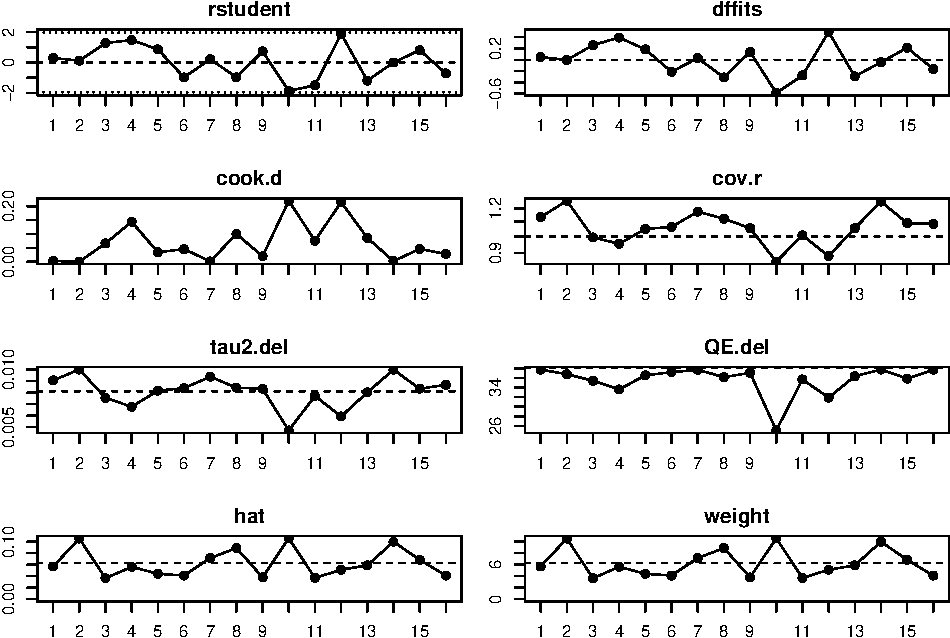
\includegraphics{Meta-analysis_files/figure-latex/unnamed-chunk-11-1.pdf}
\caption{Forest plot anotado. En esta versión agregué algunos
encabezados en español, así como estadísticos generales del modelo de
meta-análisis.}
\end{figure}

O, para una incluso más sofisticada, se puede usar la función
\texttt{viz\_forest} del paquete \texttt{metaviz}, usando la variante
\texttt{rain}.

\begin{Shaded}
\begin{Highlighting}[]
\FunctionTok{library}\NormalTok{(metaviz)}
\FunctionTok{viz\_forest}\NormalTok{(res, }
           \AttributeTok{study\_labels =} \FunctionTok{paste}\NormalTok{(dat}\SpecialCharTok{$}\NormalTok{authors, dat}\SpecialCharTok{$}\NormalTok{year, }\AttributeTok{sep =} \StringTok{", "}\NormalTok{),}
           \AttributeTok{xlab =} \StringTok{"Correlación"}\NormalTok{, }
           \AttributeTok{variant =} \StringTok{"rain"}\NormalTok{,}
           \AttributeTok{annotate\_CI =} \ConstantTok{TRUE}\NormalTok{,}
           \AttributeTok{summary\_label =} \StringTok{"Resumen"}\NormalTok{,}
           \AttributeTok{text\_size =} \FloatTok{2.6}\NormalTok{)}
\end{Highlighting}
\end{Shaded}

\begin{figure}
\centering
\includegraphics{Meta-analysis_files/figure-latex/unnamed-chunk-12-1.pdf}
\caption{\emph{Forest plot} creado con metaviz.}
\end{figure}

\hypertarget{referencias}{%
\section*{Referencias}\label{referencias}}
\addcontentsline{toc}{section}{Referencias}

\hypertarget{refs}{}
\begin{CSLReferences}{1}{0}
\leavevmode\hypertarget{ref-borensteinIdentifyingQuantifyingHeterogeneity2009}{}%
Borenstein, M., Hedges, L. V., Higgns, J. P. T., \& Rothstein, H. R.
(2009). Identifying and {Quantifying Heterogeneity}. In
\emph{Introduction to {Meta}-{Analysis}} (pp. 107--125). Wiley.
\url{https://doi.org/10.1002/9780470743386.ch16}

\leavevmode\hypertarget{ref-fisherRobumetaRpackageRobust2015}{}%
Fisher, Z., \& Tipton, E. (2015). Robumeta: {An R}-package for robust
variance estimation in meta-analysis. \emph{arXiv:1503.02220
{[}Stat{]}}. \url{http://arxiv.org/abs/1503.02220}

\leavevmode\hypertarget{ref-molloy2013}{}%
Molloy, G. J., O'Carroll, R. E., \& Ferguson, E. (2013).
Conscientiousness and Medication Adherence: A Meta-analysis.
\emph{Annals of Behavioral Medicine}, \emph{47}(1), 92--101.
\url{https://doi.org/10.1007/s12160-013-9524-4}

\leavevmode\hypertarget{ref-quintanaHowPerformMetaanalysis2021}{}%
Quintana, D. S. (2021). \emph{How to perform a meta-analysis in {R}}.
{[}Archivo de {Vídeo}{]}. YouTube. \url{https://youtu.be/lH4VZMTEZSc}.

\leavevmode\hypertarget{ref-viechtbauer2010}{}%
Viechtbauer, W. (2010). Conducting Meta-Analyses inRwith
themetaforPackage. \emph{Journal of Statistical Software}, \emph{36}(3).
\url{https://doi.org/10.18637/jss.v036.i03}

\end{CSLReferences}

\end{document}
